\chapter{Experiments and Results}

	\section{Early Experiments}
	% Capabilities of LSTM
	% - Memory: Describe binary memory example (sequence of binary digits)
	% - As classification, formula for cross-entropy loss
	% - All formulas for LSTM (gates etc.)
	% - What is the purpose of Hidden size for remembering sequence
	% - What would one possible solution for the LSTM weights?
	% - 
	
	To understand how LSTMs are used to learn from sequences of data and how their memory works, we conduct a small example for demonstration. 
	This first experiment is to show the capabilities and limitations of the LSTM.
	Can it memorize the past and use this knowledge for future outputs?
	And how far back in time can it remember?
	Does it work best for classification or regression?
	These are the main questions that are investigated in this section of the thesis.
	
	In order to tackle a machine learning problem, one needs to define three key elements:
	\begin{enumerate}
		\item The task
		\item The model
		\item The loss function
	\end{enumerate}
	We begin by defining the task. 
	The goal is to train an LSTM that remembers the last $m$ digits of a random sequence of binary digits $\vectr{x}_t \in \{0, 1\}$. 
	Thus, at time $t$ we would like the output to be the digit $\vectr{x}_{t-m}$ that was fed $m$ time steps before. 
	For example, here are two sequences of zeros and ones shifted by $m = 3$:
	\newcommand{\hlc}[2][yellow]{{%
			\colorlet{foo}{#1}%
			\sethlcolor{foo}\hl{#2}}%
	}
	\begin{center}
		\texttt{\dots01\hlc[pink]{1}\hlc[green!45]{1}\hlc[cyan!50]{0}10110\dots}
		\\
		\texttt{\dots00101\hlc[pink]{1}\hlc[green!45]{1}\hlc[cyan!50]{0}10\dots}
	\end{center}
	The first line is the input sequence and below is the desired output sequence.
	The LSTM reads the digits one by one to store them in memory and at the same time it outputs the digit from memory at time $t - 3$ as highlighted by the colors above.
	%How can we model and train this sequence-to-sequence problem?
	The first part of the model is the LSTM itself as defined in equations~\ref{eq:LSTM_recurrence} and~\ref{eq:Vanilla-LSTM-Definition}.
	Since the output can only be two numbers (zero and one), we will treat the problem as a classification task.
	To do this, we add an affine layer to shrink the size of the LSTM output $\vectr{h}_t$ down to a two-element vector
	\begin{equation}
		\vectr{z}_t = \matr{V} \vectr{h}_t + \vectr{c}.
	\end{equation}
	The last layer is the \emph{softmax} operation
	\begin{eqnarray}
		\text{softmax}(\vectr{x})_j = \frac{e^{x_{j}}}{\sum_{k=1}^{K} e^{x_{k}}},  & & j = 1, \dots, K
	\end{eqnarray}
	which is applied to $\vectr{z}_t$, where $K = 2$ in this example.
	The softmax layer forces the output to be a probability vector, which means that each entry is in the range $[0, 1]$ and all elements sum to one.
	Therefore, the output vector contains the two probabilities 
	\begin{equation*}
		\vectr{p}_t = 
		\begin{bmatrix}
			P(\vectr{o}_t = 0 \mid \vectr{x}_t, \vectr{h}_{t - 1}, \vectr{c}_{t - 1}) \\ 
			P(\vectr{o}_t = 1 \mid \vectr{x}_t, \vectr{h}_{t - 1}, \vectr{c}_{t - 1})
		\end{bmatrix}.
	\end{equation*}
	The output digit $\vectr{o}_t$ must be chosen according to the highest probability.
	A summary of the full model is shown in table~\ref{tbl:model_classification_binary_digits}.
	\begin{table}
		\small
		\begin{center}
			\begin{tabular}{|l|c|c|c|c|}
				\hline
				Layer 	& Variable 			& Input size 	& Output size 	& Parameters 			\\ \hline
				LSTM 	& $\vectr{h}_t$		& 1 			& $d$ 			& $4d(d + 1) + 4d$ 		\\ \hline
				Affine 	& $\vectr{z}_t$		& $d$ 			& 2 			& $2d + 2$ 				\\ \hline
				Softmax & $\vectr{p}_t$		& 2 			& 2 			& 0						\\ \hline
			\end{tabular}
		\end{center}
		\caption[A simple model to memorize a binary sequence]
				{A simple model to memorize a binary sequence. 
				 The variable $d$ is the hidden size of the LSTM.}
		\label{tbl:model_classification_binary_digits}
	\end{table}
	Finally, we have to define a suitable loss function. 
	For classification with softmax as the last layer, it is preferable to use the negative log-likelihood
	\begin{equation}
		L(\vectr{x}, y) = -\log\left(\vectr{x}_y\right)
	\end{equation}
	as a loss function. 
	Here, the first argument of $L$ would be replaced with the output $\vectr{p}_t$ of the network and the second argument is the ground truth label. 
	Since we are predicting the digit from $m$ time steps ago, the ground truth directly comes from the input sequence, and therefore the label $y_t$ at time $t$ is the input $\vectr{x}_{t - m}$.
	By minimizing this loss, the probability for the correct class is maximized.
	\todo{need better explanation of log-likelihood loss here}
	
	Now that task, model and loss function are defined, the model can be trained and evaluated.
	Because this experiment is completely artificial, it is possible to generate as much data as needed.
	Instead of generating many smaller sequences, one can generate a single large sequence or sample digits on-the-fly.
	
	
	\begin{figure}
		\centering
		\begin{subfigure}[b]{0.5\linewidth}
			\centering
			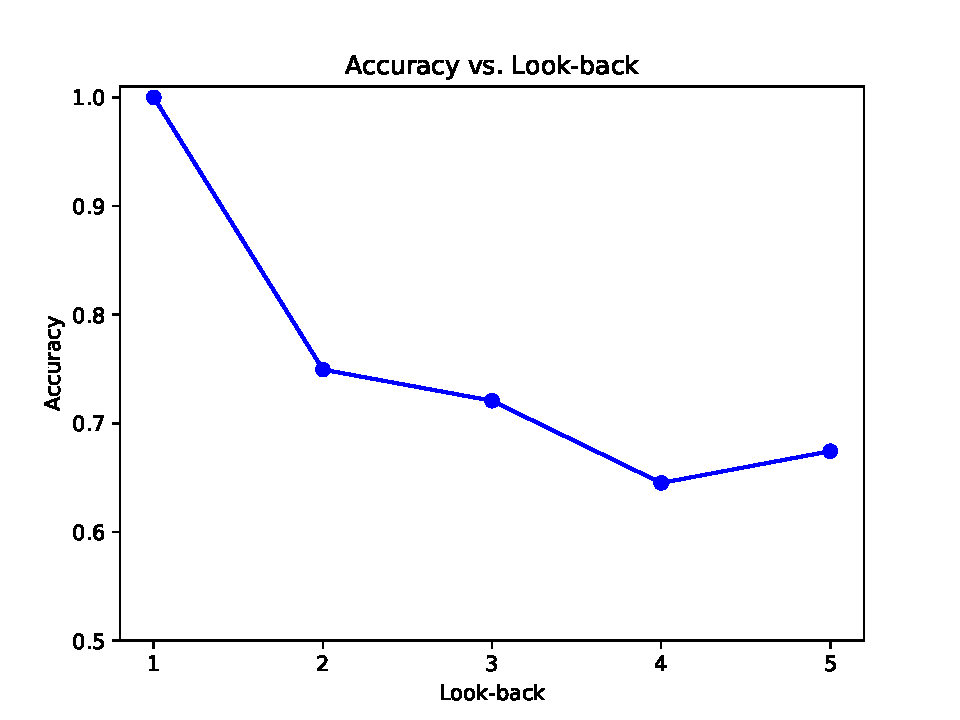
\includegraphics[width=\linewidth]{Images/Python-Plots/accuracy-vs-look-back}
			\caption{
				$d = 1, T = 50, \lambda = 0.01, N = 10^5$
				\label{fig:accuracy-vs-look-back}
			}
		\end{subfigure}%
		\begin{subfigure}[b]{0.5\linewidth}
			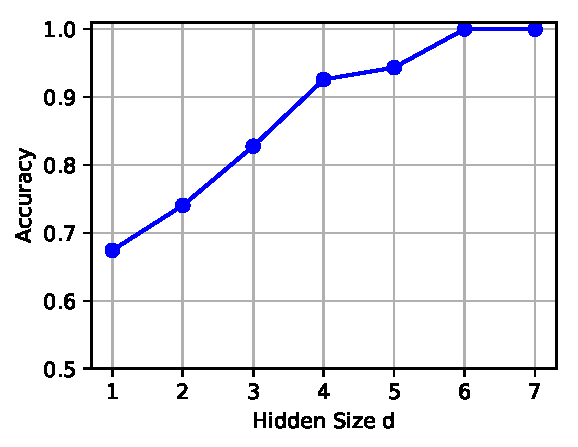
\includegraphics[width=\linewidth]{Images/Python-Plots/accuracy-vs-hidden-size}
			\caption{
				$m = 5, T = 50, \lambda = 0.01, N = 10^5$
				\label{fig:accuracy-vs-hidden-size}
			}
		\end{subfigure}
		\\
		\begin{subfigure}[b]{0.5\linewidth}
			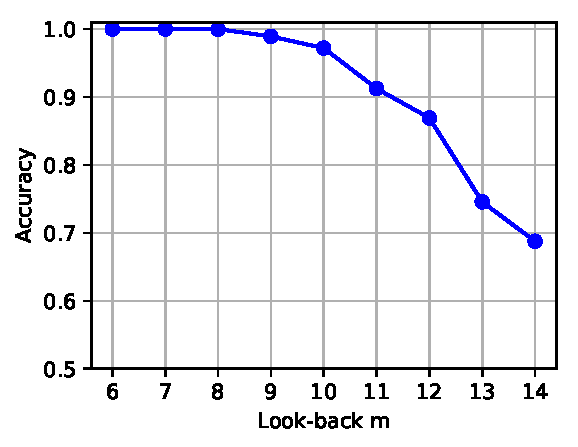
\includegraphics[width=\linewidth]{Images/Python-Plots/accuracy-vs-look-back2}
			\caption{
				$d = 50, T = 50, \lambda = 0.001, N = 10^5$
				\label{fig:accuracy-vs-look-back2}
			}
		\end{subfigure}%
		\begin{subfigure}[b]{0.5\linewidth}
			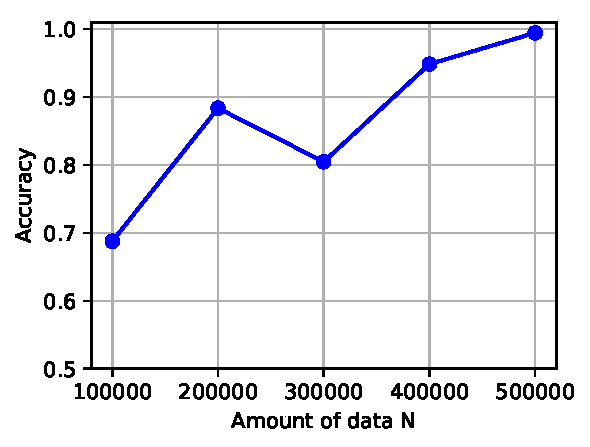
\includegraphics[width=\linewidth]{Images/Python-Plots/more-training-data}
			\caption{
				$m = 14, d = 50, T = 50, \lambda = 0.001$
				\label{fig:more-training-data}
			}
		\end{subfigure}
		\caption[Ablation study: Memorizing the past with the LSTM]
				{Accuracy on the test dataset for varying parameters while keeping others fixed. 
				 The parameters involved are the hidden size $d$, look-back $m$, BPTT $T$, training set size $N$ and learning rate $\lambda$. 
				 (a) The hidden size is too small.
				 (b) Effect of increasing the hidden size.
				 (c) Only increasing the hidden size is not enough.
				 (d) Increasing the amount of training data.}
		\label{fig:ablation-study-binary-memory}
	\end{figure}
	
	
	
	